%==============================================================================
% Sjabloon poster bachproef
%==============================================================================
% Gebaseerd op document class `a0poster' door Gerlinde Kettl en Matthias Weiser
% Aangepast voor gebruik aan HOGENT door Jens Buysse en Bert Van Vreckem

\documentclass[a0,portrait]{hogent-poster}

% Info over de opleiding
\course{Bachelorproef}
\studyprogramme{toegepaste informatica}
\academicyear{2024-2025}
\institution{Hogeschool Gent, Valentin Vaerwyckweg 1, 9000 Gent}

% Info over de bachelorproef
\title{Alternatieven voor Dropbox bij Aquarius Zwemclub Lebbeke.}
\subtitle{Een onderzoek naar cloudopslag.}
\author{Luka Deserranno}
\email{Luka.Deserranno@student.hogent.be}
\supervisor{Sonia VanderMeersch}
\cosupervisor{Thomas Aelbrecht (Aquarius Zwemclub Lebbeke)}

% Indien ingevuld, wordt deze informatie toegevoegd aan het einde van de
% abstract. Zet in commentaar als je dit niet wilt.
\keywords{Cloudopslag, Angular, Node.js, Toegangsbeheer, DigitalOcean Spaces}

\begin{document}

\maketitle

\begin{abstract}
Bestandenbeheer bij kleine sportverenigingen blijft een veelvoorkomend knelpunt. Diensten zoals Dropbox en OneDrive worden vaak ingezet, maar kampen met belangrijke beperkingen: ze vereisen extra accounts, bieden beperkte controle over toegangsrechten en integreren moeilijk met bestaande digitale omgevingen.

Ook Aquarius Zwemclub Lebbeke (AZL) ondervond deze problemen. Lesgevers hadden geen uniforme toegang tot bestanden, toegangsrechten waren moeilijk beheersbaar en het beheer verliep grotendeels manueel. Dit leidde tot inefficiëntie en frustratie bij de gebruikers.

In deze bachelorproef werd onderzocht of het mogelijk is een cloudopslagoplossing te implementeren die:
\begin{itemize}
\item Naadloos integreert in het bestaande platform van AZL
\item Fijnmazige toegangscontrole per gebruiker en mapniveau mogelijk maakt
\item Beschikbaar is zonder dat lesgevers extra accounts moeten aanmaken
\item Voldoende schaalbaar en toekomstbestendig is
\end{itemize}

Als oplossing werd gekozen voor een infrastructuur gebaseerd op DigitalOcean, waarbij een eigen cloudomgeving werd opgezet met een intuïtieve gebruikersinterface, rechtstreeks toegankelijk via het interne platform van AZL. Door gebruik te maken van open-source componenten en API-koppelingen werd een oplossing gebouwd die volledig aangepast is aan de noden van de club.

Een proof of concept werd ontwikkeld en getest binnen de bestaande IT-omgeving. De resultaten tonen aan dat deze oplossing het beheer van bestanden sterk vereenvoudigt, de veiligheid verhoogt door betere toegangscontrole, en de gebruikservaring voor lesgevers aanzienlijk verbetert.

Deze aanpak biedt niet enkel voordelen voor AZL, maar kan ook dienen als model voor andere kleine sportorganisaties met gelijkaardige uitdagingen.

\end{abstract}

\begin{multicols}{2} % This is how many columns your poster will be broken into, a portrait poster is generally split into 2 columns

\section{Probleemstelling \& Doelstelling}  

Aquarius Zwemclub Lebbeke (AZL) maakte tot voor kort gebruik van Dropbox voor het delen van lesmateriaal tussen lesgevers. Dit leidde echter tot structurele problemen: verouderde toegangsrechten, gebrek aan integratie met de bestaande webapplicatie en beperkte toegankelijkheid voor lesgevers zonder Dropbox-account.

Het doel van deze bachelorproef was om een cloudopslagoplossing te ontwikkelen die:
\begin{itemize}
  \item veilig en gebruiksvriendelijk is;
  \item naadloos integreert met de bestaande Angular/Node.js-infrastructuur van AZL;
  \item en fijnmazig toegangsbeheer ondersteunt zonder dat extra accounts nodig zijn.
\end{itemize}

Op basis van een vergelijkende analyse werd gekozen voor een oplossing gebaseerd op DigitalOcean Spaces, in combinatie met een aangepaste gebruikersinterface.

\section{Uitwerking}

Om na te gaan of de gekozen cloudopslagoplossing voldoet aan de noden van Aquarius Zwemclub Lebbeke (AZL), 
werd een proof of concept ontwikkeld en getest binnen de bestaande infrastructuur. De oplossing bestaat uit een op maat gemaakte 
integratie tussen DigitalOcean Spaces (S3-compatibele objectopslag) en de bestaande Angular/Node.js-webapplicatie van AZL. 
Hierbij werd een fijnmazig toegangsbeheersysteem geïmplementeerd waarbij per gebruiker en per bestand of map specifieke rechten 
kunnen worden toegekend (lezen, schrijven, beheren).

De backend genereert veilige, tijdelijke toegangstokens (pre-signed URLs), waarmee lesgevers via de frontend bestanden kunnen uploaden of downloaden 
zonder dat zij direct toegang hebben tot de cloudopslag zelf. Daarnaast werd een gebruiksvriendelijke interface ontwikkeld waarin lesgevers bestanden 
kunnen beheren binnen hun toegestane mappen.

\begin{center}
  \captionsetup{type=figure}
  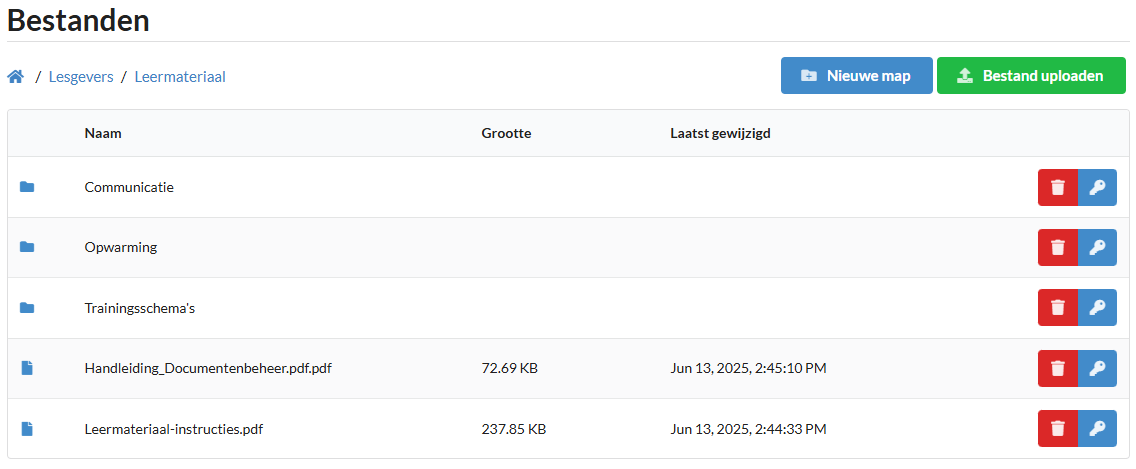
\includegraphics[width=1.0\linewidth]{file-manager.png}
  \captionof{figure}{Screenshot van de geïmplementeerde UI-component voor bestandsbeheer. Lesgevers krijgen gepersonaliseerde toegang tot mappen en bestanden via een geïntegreerd systeem met fijnmazige toegangscontrole.}
\end{center}

\section{Conclusies \& Aanbevelingen}  

Het proof of concept toont aan dat een op DigitalOcean gebaseerde cloudopslagoplossing, gekoppeld aan een aangepaste Angular-interface, perfect inspeelt op de behoeften van AZL. Lesgevers krijgen eenvoudig toegang tot documenten, zonder bijkomende accounts, en de beheerder beschikt over nauwkeurige controle over toegangsrechten.

De oplossing draagt bij aan:
\begin{itemize}
  \item efficiënter beheer van lesmateriaal;
  \item een gebruiksvriendelijker platform voor alle betrokkenen;
  \item en een lagere administratieve werklast.
\end{itemize}

Aanbevolen wordt om het prototype verder uit te rollen binnen AZL en te overwegen het concept te hergebruiken bij gelijkaardige verenigingen.

\section{Toekomstig onderzoek}

De oplossing die in deze bachelorproef werd ontwikkeld voor Aquarius Zwemclub Lebbeke, 
biedt een waardevolle blauwdruk voor andere kleine sportverenigingen die kampen met gelijkaardige uitdagingen rond documentenbeheer, 
toegangsrechten en gebruiksvriendelijkheid. Veel verenigingen beschikken over beperkte IT-kennis en infrastructuur, 
waardoor generieke oplossingen zoals Dropbox of OneDrive vaak onvoldoende afgestemd zijn op hun specifieke werking. 
Een interessante piste voor toekomstig onderzoek is het generaliseren van deze oplossing tot een flexibel en schaalbaar platform voor sportclubs. 
Dit platform zou modulaire componenten kunnen bevatten voor toegangsbeheer, cloudopslag en koppelingen met bestaande websites of ledenbeheer. 
Door gebruik te maken van S3-compatibele opslag zoals DigitalOcean Spaces, gecombineerd met een intuïtieve gebruikersinterface, 
kunnen clubs zonder technische voorkennis een veilige en geïntegreerde digitale werkomgeving opzetten. 
Verder onderzoek kan ook peilen naar automatisering van rechtenbeheer op basis van ledenrollen, gebruik van mobiele toegang, 
en optimalisatie van kostenstructuren bij grootschaliger gebruik. Zo kan het huidige proof of concept evolueren tot een breder 
inzetbare tool die bijdraagt aan digitale professionalisering binnen de sportsector.

\end{multicols}
\end{document}